Die Übergangsfunktion stellt die Veränderung des Signals innerhalb des Systems als Funktion dar. Diese
kann durch Integrieren aus der Gewichtsfunktion (später dargestellt) gebildet werden. Dafür nutzt man wie
in den folgenden Abbildungen dargestellt den Laplace-Bereich, da nicht alle Funktionen einfach integriert
werden können.
\vspace*{0.5cm}
\begin{figure}[H]
    \begin{center}
        \fbox{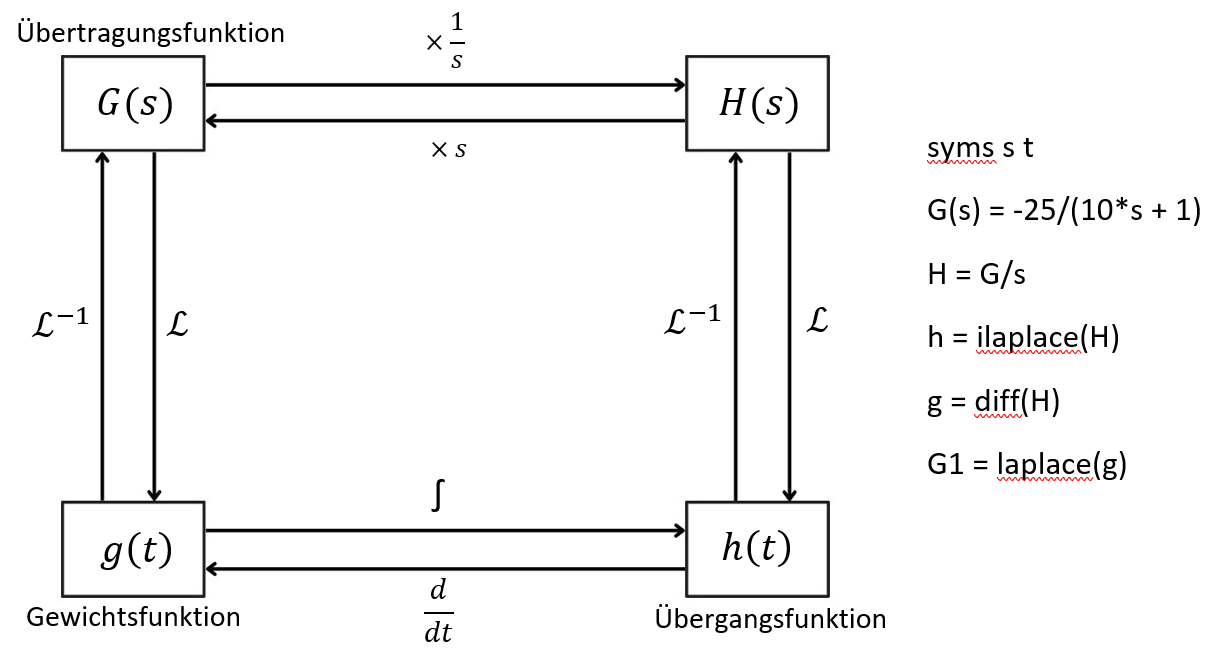
\includegraphics[width=13cm]{image/funktionen-fertig.png}}
    \end{center}
\end{figure}
\vspace*{0.5cm}